\documentclass{article}
\usepackage[british]{babel}
\usepackage{../lib/tex/naproche}
\documentclass[12pt,oneside]{book}

\usepackage[foundations]{../../lib/tex/naproche}
\usepackage{../../lib/tex/libraries}
\usepackage{graphicx}
\usepackage{float}
\usepackage{caption}
\usepackage{footnote}

\makesavenoteenv{tabular} % Make footnotes work in tabular environments


\title{Foundations of Mathematics}
\author{Marcel Schütz}
\date{2022}

\begin{document}
  \maketitle

  \tableofcontents

  \begin{figure}[H]
    \centering
    \fbox{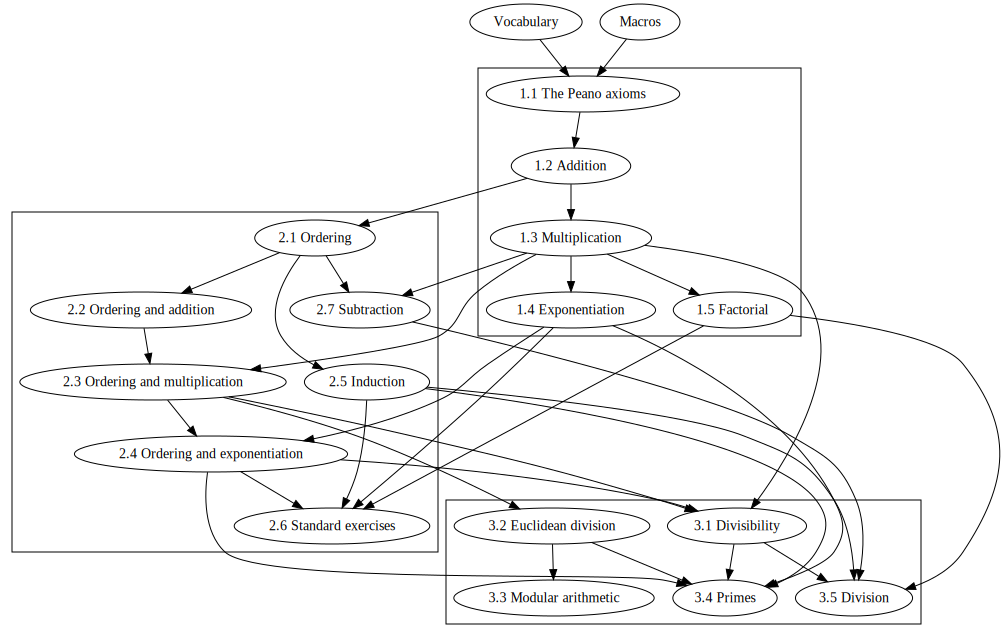
\includegraphics[width=0.9\linewidth]{./dependency-graph/graph.png}}
    \caption*{Interdependencies of the chapters}
  \end{figure}


  \section*{Introduction}

  This is a library providing a foundation of mathematics based on a
  Kelley-Morse like class theory with urelements.
  It introduces common operations on classes like unions or intersections
  (\cref{chapter:classes}) together with detailed proofs of their algebraic
  properties (\cref{chapter:computation-laws-for-classes}), the symmetric
  difference of two classes (\cref{chapter:symmetric-difference}) and the
  notions of ordered pairs and Cartesian products
  (\cref{chapter:pairs-and-products}) as well as proofs of the algebraic
  properties of the latter (\cref{chapter:computation-laws-for-products}).
  Moreover, it provides common operations on maps (\cref{chapter:maps}), various
  properties of images and preimages (\cref{chapter:image-and-preimage}) and the
  notions of injectivity, surjectivity, bijectivity
  (\cref{chapter:injections-surjections-bijections}) and invertibility of maps
  (\cref{chapter:invertible-maps}).
  The library provides an axiom system characterizing sets (\cref{chapter:sets})
  and, furthermore, it covers the notions of binary relations
  (\cref{chapter:binary-relations}), fixed-points of subset preserving maps
  (\cref{chapter:fixed-points}), including and equinumerosity
  (\cref{chapter:equinumerosity}).

  As two famous results it includes the Knaster-Tarski fixed point theorem
  (\cref{FOUNDATIONS_12_8420450166112256}) and the Cantor-Schröder-Bernstein
  theorem (\cref{FOUNDATIONS_13_1913663275401216}).

  \paragraph*{Usage.}
  At the very beginning of each chapter you can find the name of its source
  file, e.g. \path{foundations/sections/01_classes.ftl.tex} for
  \cref{chapter:classes}. This filename can be used to import the chapter via
  \Naproche's \texttt{readtex} instruction to another ForTheL text, e.g.:
  \begin{center}
    \verb`[readtex \path{foundations/sections/01_classes.ftl.tex}]`
  \end{center}

  \paragraph*{Checking times.}
  The checking times for each of the chapters may vary from computer to
  computer, but on mid-range hardware they are likely to be similar to those
  given in table below:

  \begin{center}
    \begin{tabular}{c|c|c}

      & \multicolumn{2}{c}{\textbf{Checking time}}
      \\
      \textbf{Chapter}
      & \textbf{without dependencies}     & \textbf{with dependencies}
      \\ \hline
      \ref{chapter:classes}
      & 00:04 min                         & 00:04 min
      \\
      \ref{chapter:computation-laws-for-classes}
      & 00:12 min                         & 00:16 min
      \\
      \ref{chapter:symmetric-difference}
      & 00:32 min                         & 00:48 min
      \\
      \ref{chapter:pairs-and-products}
      & 00:08 min                         & 00:12 min
      \\
      \ref{chapter:computation-laws-for-products}
      & 01:36 min                         & 01:56 min
      \\
      \ref{chapter:maps}
      & 01:13 min                         & 01:25 min
      \\
      \ref{chapter:image-and-preimage}
      & 01:28 min                         & 02:53 min
      \\
      \ref{chapter:injections-surjections-bijections}
      & 00:38 min                         & 02:03 min
      \\
      \ref{chapter:invertible-maps}
      & 02:20 min                         & 04:23 min
      \\
      \ref{chapter:sets}
      & 02:17 min                         & 06:40 min
      \\
      \ref{chapter:binary-relations}
      & 00:14 min                         & 06:54 min
      \\
      \ref{chapter:fixed-points}
      & 00:33 min                         & 07:13 min
      \\
      \ref{chapter:equinumerosity}
      & 01:48 min                         & 09:01 min
    \end{tabular}
  \end{center}


  \subfile{sections/01_classes.ftl.tex}
  \subfile{sections/02_computation-laws-for-classes.ftl.tex}
  \subfile{sections/03_symmetric-difference.ftl.tex}
  \subfile{sections/04_pairs-and-products.ftl.tex}
  \subfile{sections/05_computation-laws-for-products.ftl.tex}
  \subfile{sections/06_maps.ftl.tex}
  \subfile{sections/07_image-and-preimage.ftl.tex}
  \subfile{sections/08_injections-surjections-bijections.ftl.tex}
  \subfile{sections/09_invertible-maps.ftl.tex}
  \subfile{sections/10_sets.ftl.tex}
  \subfile{sections/11_binary-relations.ftl.tex}
  \subfile{sections/12_fixed-points.ftl.tex}
  \subfile{sections/13_equinumerosity.ftl.tex}
\end{document}

\documentclass[12pt,oneside]{book}

\usepackage[utf8]{inputenc}
\usepackage[english]{babel}

\usepackage{../meta-inf/lib/naproche-logo}
\usepackage{../meta-inf/lib/naproche}
\usepackage{../meta-inf/lib/libraries}
\usepackage{naproche}
\usepackage{naproche-libraries}
\renewcommand\libarchive{Preliminaries}
\usepackage{naproche}
\usepackage{naproche-libraries}
\renewcommand\libarchive{Preliminaries}

\usepackage{xr}
\externaldocument{../foundations/foundations}

\usepackage{graphicx}
\usepackage{float}
\usepackage{caption}
\usepackage[nobottomtitles]{titlesec}


\title{Set theory}
\author{Marcel Schütz}
\date{2022}

\begin{document}
  \maketitle

  \tableofcontents

  \paragraph*{}
  \begin{figure}[H]
    \centering
    \fbox{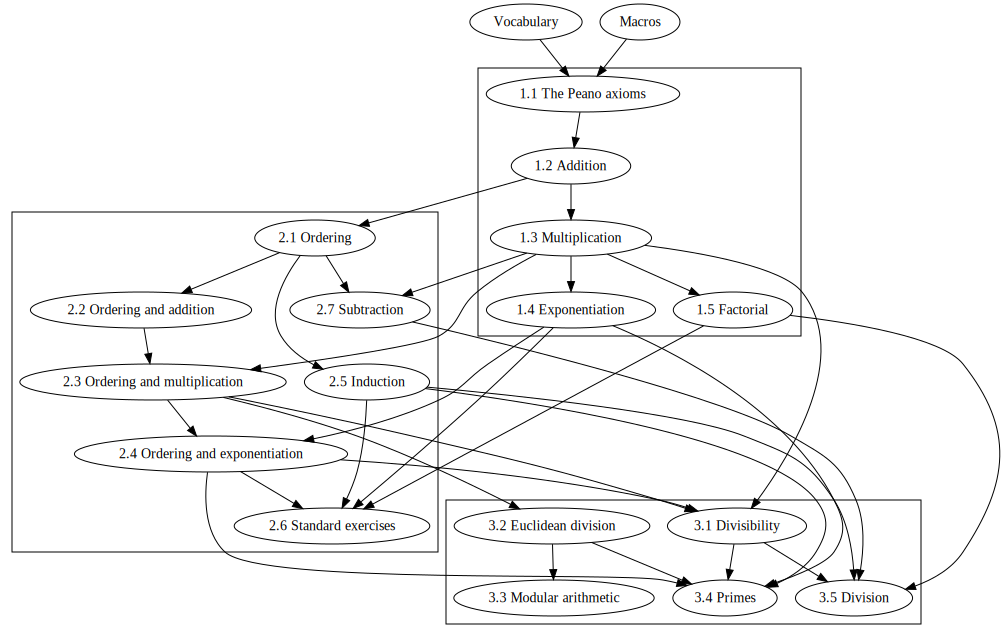
\includegraphics[width=0.9\textwidth]{./dependency-graph/graph.png}}
    \caption*{Interdependencies of the chapters}
  \end{figure}

  \section*{Introduction}

  This is a library providing basic results from undergraduate-level set theory.
  It introduces the notion of transitive classes
  (\cref{chapter:transitive-classes}), defines the notion of ordinal numbers
  (\cref{chapter:ordinals}) and as a special case of the latter introduces the
  set $\omega$ of finite ordinals (\cref{chapter:finite-ordinals}).
  Moreover, this library provides a formalization of the ordinal recursion
  theorem (\cref{chapter:recursion}) which is used to prove Zermelo's
  well-ordering theorem (\cref{chapter:zermelo}), on the basis of which the
  notion of cardinal numbers is introduced (\cref{chapter:cardinals}).
  Furthermore, some results about finite and infinite sets are given
  (\cref{chapter:finite-and-infinite-sets}).

  \paragraph*{Usage.}
  At the very beginning of each chapter you can find the name of its source
  file, e.g. \path{set-theory/sections/01_transitive-classes.ftl.tex} for
  \cref{chapter:transitive-classes}.
  This filename can be used to import the chapter via \Naproche's
  \texttt{readtex} instruction to another ForTheL text, e.g.:
  \begin{center}
    \verb`[readtex \path{set-theory/sections/01_transitive-classes.ftl.tex}]`
  \end{center}

  \paragraph*{Checking times.}
  The checking times for each of the chapters may vary from computer to
  computer, but on mid-range hardware they are likely to be similar to those
  given in table below:

  \begin{center}
    \begin{tabular}{c|c|c}

      & \multicolumn{2}{c}{\textbf{Checking time}}
      \\
      \textbf{Chapter}
      & \textbf{without dependencies}     & \textbf{with dependencies}
      \\ \hline
      \ref{chapter:transitive-classes}
      & 00:20 min                         & 07:00 min
      \\
      \ref{chapter:ordinals}
      & 03:20 min                         & 10:30 min
      \\
      \ref{chapter:finite-ordinals}
      & 01:15 min                         & 11:45 min
      \\
      \ref{chapter:recursion}
      & 04:05 min                         & 14:35 min
      \\
      \ref{chapter:zermelo}
      & 04:45 min                         & 21:40 min
      \\
      \ref{chapter:cardinals}
      & 05:10 min                         & 26:50 min
      \\
      \ref{chapter:finite-and-infinite-sets}
      & 10:50 min                         & 38:55 min
    \end{tabular}
  \end{center}

  \subfile{sections/01_transitive-classes.ftl.tex}
  \subfile{sections/02_ordinals.ftl.tex}
  \subfile{sections/03_finite-ordinals.ftl.tex}
  \subfile{sections/04_recursion.ftl.tex}
  \subfile{sections/05_well-ordering-theorem.ftl.tex}
  \subfile{sections/06_cardinals.ftl.tex}
  \subfile{sections/07_finite-and-infinite-sets.ftl.tex}
\end{document}


\usepackage[backend=bibtex]{biblatex}
\usepackage{csquotes}
\addbibresource{meta-inf/lib/bibliography}

\title{Transfinite Recursion Theorem}
\author{\Naproche formalization: \vspace{0.5em} \\
Marcel Schütz}
\date{2024}

\begin{document}
  \maketitle

  \begin{imports}
    \begin{forthel}
      %[prove off][check off]
      [readtex \path{libraries/source/set-theory/transfinite-induction.ftl.tex}]
      [readtex \path{libraries/source/set-theory/recursive-maps.ftl.tex}]
      %[prove on][check on]
    \end{forthel}
  \end{imports}
  
  \noindent This is a formalization of the \emph{Transfinite Recursion Theorem}
  (cf. \cite{Koepke2018}).
  It states that for any map $G : A^{< \infty} \to A$, where $A^{< \infty}$
  denotes the class of all maps $\alpha \to A$ for some ordinal $\alpha$, there
  exists a unique map $F: \Ord \to A$ that is \emph{recursive regarding} $G$,
  i.e. \[F(\alpha) = G(F \restriction \alpha)\] for all ordinals $\alpha$.

  \begin{forthel}
    \begin{lemma*}[Coincidence Lemma]\label{coincidence}
      Let $A$ be a class and $G$ be a map from $A^{< \infty}$ to $A$.
      Let $H, H'$ be maps to $A$ that are recursive regarding $G$.
      Then \[ H(\alpha) = H'(\alpha) \] for all $\alpha \in \dom(H) \cap \dom(H')$.
    \end{lemma*}
    \begin{proof}
      Define $\Phi = \{ \alpha \in \Ord \mid$ if
      $\alpha \in \dom(H) \cap \dom(H')$ then $H(\alpha) = H'(\alpha) \}$.

      For all ordinals $\alpha$ if every ordinal less than $\alpha$ lies in $\Phi$ then $\alpha \in \Phi$. \\
      Proof.
        Let $\alpha \in \Ord$.
        Assume that every $y \in \alpha$ lies in $\Phi$.

        Let us show that if $\alpha \in \dom(H) \cap \dom(H')$ then
        $H(\alpha) = H'(\alpha)$.
          Suppose $\alpha \in \dom(H) \cap \dom(H')$.
          Then $\alpha \subseteq \dom(H), \dom(H')$.
          Indeed $\dom(H)$ and $\dom(H')$ are transitive classes.
          Hence for all $y \in \alpha$ we have $y \in \dom(H) \cap \dom(H')$.
          Thus $H(y) = H'(y)$ for all $y \in \alpha$.
          Therefore $H \restriction \alpha = H' \restriction \alpha$.
          $H$ and $H'$ are recursive regarding $G$.
          We have $H \restriction \alpha, H' \restriction \alpha \in A^{< \infty}$.
          Hence $H(\alpha)
            = G(H \restriction \alpha)
            = G(H' \restriction \alpha)
            = H'(\alpha)$.
        End.

        Thus $\alpha \in \Phi$.
      Qed.

      [prover vampire]
      Then $\Phi$ contains every ordinal (by \printref{SET_THEORY_02_8493935460614144}).
      Therefore we have $H(\alpha) = H'(\alpha)$ for all $\alpha \in \dom(H) \cap \dom(H')$.
    \end{proof}
  \end{forthel}

  \begin{forthel}
    \begin{theorem*}[Transfinite Recursion Theorem: Existence]\label{recursion_existence}
      Let $A$ be a class and $G$ be a map from $A^{< \infty}$ to $A$.
      Then there exists a map $F$ from $\Ord$ to $A$ that is recursive regarding $G$.
    \end{theorem*}
    \begin{proof}
      Every ordinal is contained in the domain of some map $H$ to $A$ such that $H$ is recursive regarding $G$. \\
      Proof.
        Define \[ \Phi = \class{\alpha \in \Ord | \classtext{$\alpha$ is contained in the domain of some map to $A$ that is recursive regarding $G$}}. \]

        Let us show that for every ordinal $\alpha$ if every ordinal less than $\alpha$ lies in $\Phi$ then $\alpha \in \Phi$.
          Let $\alpha$ be an ordinal.
          Assume that every ordinal less than $\alpha$ lies in $\Phi$.
          Then for all $y \in \alpha$ there exists a map $h$ to $A$ such that $h$ is recursive regarding $G$ and $y \in \dom(h)$.
          Define $H'(y) =$ ``choose a map $h$ to $A$ such that $h$ is recursive regarding $G$ and $y \in \dom(h)$ in $h(y)$'' for $y \in \alpha$.
          Then $H'$ is a map from $\alpha$ to $A$.
          We have $H' = H' \restriction \alpha$.
          Define \[ H(\beta) =
            \begin{cases}
              H'(\beta)                 & : \beta < \alpha \\
              G(H' \restriction \beta)  & : \beta = \alpha
            \end{cases} \]
          for $\beta \in \succ(\alpha)$.
          
          Let us show that $H \restriction \beta \in A^{< \infty}$ for all $\beta \in \dom(H)$.
            Let $\beta \in \dom(H)$.
            $\dom(H \restriction \beta) = \beta$ and $(H \restriction \beta)(b) = H(b)$ for all $b \in \beta$.
            $H(b) \in A$ for all $b \in \beta$.
            Hence $H \restriction \beta$ is a map from $\beta$ to $A$.
          End.

          (a) $\dom(H)$ is a transitive subclass of $\Ord$.

          (b) For all $\beta \in \dom(H)$ we have $H(\beta) = G(H \restriction \beta)$. \\
          Proof.
            Let $\beta \in \dom(H)$.
            Then $\beta < \alpha$ or $\beta = \alpha$.

            Case $\beta < \alpha$.
              Choose a map $h$ to $A$ such that $h$ is recursive regarding $G$ and $\beta \in \dom(h)$ and $H'(\beta) = h(\beta)$.

              Let us show that for all $y \in \beta$ we have $h(y) = H(y)$.
                Let $y \in \beta$.
                Then $H(y) = H'(y)$.
                Choose a map $h'$ to $A$ such that $h'$ is recursive regarding $G$ and $y \in \dom(h')$ and $H'(y) = h'(y)$.
                [prover vampire]
                Then $h'(y) = h(y)$ (by \nameref{coincidence}).
                Indeed $y \in \dom(h) \cap \dom(h')$.
              End.

              Hence $h \restriction \beta = H \restriction \beta$.
              Thus $H(\beta)
                = H'(\beta)
                = h(\beta)
                = G(h \restriction \beta)
                = G(H \restriction \beta)$.
            End.

            Case $\beta = \alpha$.
              We have $H \restriction \alpha = H' \restriction \alpha$.
            End.
          Qed.

          Hence $H$ is a map to $A$ such that $H$ is recursive regarding $G$ and $\alpha \in \dom(H)$.
          Thus $\alpha \in \Phi$.
        End.

        [prover vampire]
        Therefore $\Phi$ contains every ordinal (by \printref{SET_THEORY_02_8493935460614144}).
        Consequently every ordinal is contained in the domain of some map $H$ to $A$ such that $H$ is recursive regarding $G$.
      Qed.

      Define $F(\alpha) =$ ``choose a map $H$ to $A$ such that $H$ is recursive regarding $G$ and $\alpha \in \dom(H)$ in $H(\alpha)$'' for $\alpha \in \Ord$.
      Then $F$ is a map from $\Ord$ to $A$.

      $F$ is recursive regarding $G$. \\
      Proof.
        (a) $\dom(F)$ is a transitive subclass of $\Ord$.

        (b) For all $\alpha \in \Ord$ we have $F(\alpha) = G(F \restriction \alpha)$. \\
        Proof.
          Let $\alpha \in \Ord$.
          Choose a map $H$ to $A$ such that $H$ is recursive regarding $G$ and $\alpha \in \dom(H)$ and $F(\alpha) = H(\alpha)$.

          Let us show that $F(\beta) = H(\beta)$ for all $\beta \in \alpha$.
            Let $\beta \in \alpha$.
            Choose a map $H'$ to $A$ such that $H'$ is recursive regarding $G$ and $\beta \in \dom(H')$ and $F(\beta) = H'(\beta)$.
            [prover vampire]
            Then $H(\beta) = H'(\beta)$ (by \nameref{coincidence}).
            Indeed $\beta \in \dom(H) \cap \dom(H')$.
            Therefore $F(\beta) = H'(\beta)$.
          End.

          Hence $H \restriction \alpha = F \restriction \alpha$.
          Thus $F(\alpha)
            = H(\alpha)
            = G(H \restriction \alpha)
            = G(F \restriction \alpha)$.
        Qed.
      Qed.
    \end{proof}
  \end{forthel}

  \begin{forthel}
    \begin{theorem*}[Transfinite Recursion Theorem: Uniqueness]\label{recursion_uniqueness}
      Let $A$ be a class and $G$ be a map from $A^{< \infty}$ to $A$.
      Let $F, F'$ be maps from $\Ord$ to $A$ that are recursive regarding $G$.
      Then $F = F'$.
    \end{theorem*}
    \begin{proof}
      [prover vampire]
      $F$ and $F'$ are recursive regarding $G$.
      Then $F(\alpha) = F'(\alpha)$ for all $\alpha \in \dom(F) \cap \dom(F')$ (by \nameref{coincidence}).
      We have $\dom(F) = \Ord = \dom(F')$.
      Hence $F(\alpha) = F'(\alpha)$ for all $\alpha \in \Ord$.
      Thus $F = F'$.
    \end{proof}
  \end{forthel}

  As a corollary of the transfinite recursion theorem we get that we can
  define maps recursively on the ordinals by case distinction:
  For given maps $G : \Ord \times A \to A$ and
  $H : \Ord \times A^{< \infty} \to A$ and an element $a \in A$ we can define
  a map $F : \Ord \to A$ by
  \begin{itemize}
    \item $F(0) = a$,
    \item $F(\succ(\alpha)) = G(\alpha, F(\alpha))$, and
    \item $F(\lambda) = H(\lambda, F \restriction \lambda)$
      for any limit ordinal $\lambda$.
  \end{itemize}

  To establish the well-formedness of the conclusion of that corollary in
  \linebreak
  \Naproche, we need two additional lemmas:

  \begin{forthel}
    \begin{lemma*}
      Let $A$ be a class and $\alpha$ be an ordinal and $F : \Ord \to A$.
      Then $(\alpha, F(\alpha)) \in \Ord \times A$.
    \end{lemma*}

    \begin{lemma*}
      Let $A$ be a class and $\lambda$ be a limit ordinal and $F : \Ord \to A$.
      Then $(\lambda, F \restriction \lambda) \in \Ord \times A^{< \infty}$.
    \end{lemma*}
  \end{forthel}

  \begin{forthel}
    \begin{corollary*}\label{recursion}
      Let $A$ be a class.
      Let $a \in A$ and $G : \Ord \times A \to A$ and $H : \Ord \times A^{< \infty} \to A$.
      Then there exists a map $F$ from $\Ord$ to $A$ such that
      \[ F(0) = a \]
      and for all ordinals $\alpha$ we have
      \[ F(\succ(\alpha)) = G(\alpha, F(\alpha)) \]
      and for all limit ordinals $\lambda$ we have
      \[ F(\lambda) = H(\lambda, F \restriction \lambda). \]
    \end{corollary*}
    \begin{proof}
      $(\pred(\dom(f)), f(\pred(\dom(f)))) \in \Ord \times A$ for all $f \in A^{< \infty}$ such that $\dom(f)$ is a successor ordinal.

      Define  \[ J(f) =
        \begin{cases}
          a
          & : \dom(f) = 0
          \\
          G(\pred(\dom(f)), f(\pred(\dom(f))))
          & : \text{$\dom(f)$ is a successor ordinal}
          \\
          H(\dom(f), f)
          & : \text{$\dom(f)$ is a limit ordinal}
        \end{cases} \]
      for $f \in A^{< \infty}$.

      Then $J$ is a map from $A^{< \infty}$ to $A$.
      Indeed we can show that for any $f \in A^{< \infty}$ we have $J(f) \in A$.
        Let $f \in A^{< \infty}$.
        Take $\alpha \in \Ord$ such that $f : \alpha \to A$.
        If $\alpha = 0$ then $J(f) = a \in A$.
        If $\alpha$ is a successor ordinal then $J(f) =
        G(\pred(\alpha), f(\pred(\alpha))) \in A$.
        [prover vampire]
        If $\alpha$ is a limit ordinal then $J(f) = H(\alpha, f) \in A$.
      End.

      Hence we can take a map $F$ from $\Ord$ to $A$ that is recursive regarding $J$.
      Then $F \restriction \alpha \in A^{< \infty}$ for any ordinal $\alpha$.

      (1) $F(0) = a$. \\
      Proof.
        $F(0)
          = J(F \restriction 0)
          = a$.
      Qed.

      (2) $F(\succ(\alpha)) = G(\alpha, F(\alpha))$ for all ordinals $\alpha$. \\
      Proof.
        Let $\alpha$ be an ordinal.
        Then $F(\succ(\alpha))
          = J(F \restriction \succ(\alpha))
          = G(\pred(\succ(\alpha)), (F \restriction \succ(\alpha))(\pred(\succ(\alpha))))
          = G(\alpha, (F \restriction \succ(\alpha))(\alpha))
          = G(\alpha, F(\alpha))$.
      Qed.

      (3) $F(\lambda) = H(\lambda, F \restriction \lambda)$ for all limit ordinals $\lambda$. \\
      Proof.
        Let $\lambda$ be a limit ordinal.
        Then $F(\lambda)
          = J(F \restriction \lambda)
          = H(\lambda, F \restriction \lambda)$.
      Qed.

      Hence the thesis (by 1, 2, 3).
    \end{proof}
  \end{forthel}

  \printbibliography
\end{document}
